% **Problems**

% - Contains a bit of background info about NB-IoT which should not be there
% - Mixes sensor readings w/ data transmissions a bit

% **Needs to contain**

% - Motivations for why we need certain requirements
% - Maybe some behavior graphs for clarification
% - What issues can arise and what we want to do about it.

% **Structure**

% - Summary of subsections at the top
% - Data transmission
% - Sensor readings
% - Sensor failure
% - Sensor disconnect

In this section we will discuss some the software requirements imposed on the IoT-enabled scale device that will be implemented, and what behavior we wish to see from the device in the case of different scenarios. These areas were chosen because of their relative simple nature, as well as their relevance to other similar devices. The purpose of these requirements is to emulate the constraints placed on devices in the real world, specifically an all-purpose IoT-scale that Vetek could use in a pilot project for evaluation and future iterations. 

There are no specific requirements set for the hardware implementation. Any additional requirements in terms of energy consumption, sizing, etc. would be too vast for the scope of this paper. 

\section{Data Polling Rate}
In most IoT devices the relevant data is provided by some form of sensor, whether it be a scale, thermometer or something entirely different \cite{what_is_iot}. The type of sensor being used has a huge impact on the IoT device, especially when considering that they have to be powered by the same energy source. The simplest way of deciding when to poll data from a sensor is to let it do so at a fixed and constant rate, often enough to be relevant, and seldom enough as to not waste precious energy. However, if within the context of the application we can conclude that no data needs to be polled (for a while), then subsequently no data will need to be sent, and thus we save energy on both ends of the system. For some applications there might even be longer periods of downtime where it is not relevant to conduct monitoring on the given sensor, \eg during nighttime, closing hours, etc. Another interesting angle is modifying the polling rate depending on the data itself. A simple example of a behavior would be to have a slower polling rate at stable values, and increase it when experiencing large enough changes. Given the conditions of an IoT device powered by batteries, it is not unreasonable to assume that readings might not always be accurate at times. Depending on the sensor, spikes and drops of false values might occur, and not taking these scenarios into account would be prudent. 

In this paper, we want the device to change its polling rate depending on the data values, such that the rate increases at periods of activity and change, and lower the rate when the data stabilizes around a given value. The device should also try to take false data values into account.

\begin{figure}[H]
\centering
	\begin{subfigure}[b]{0.3\textwidth}
    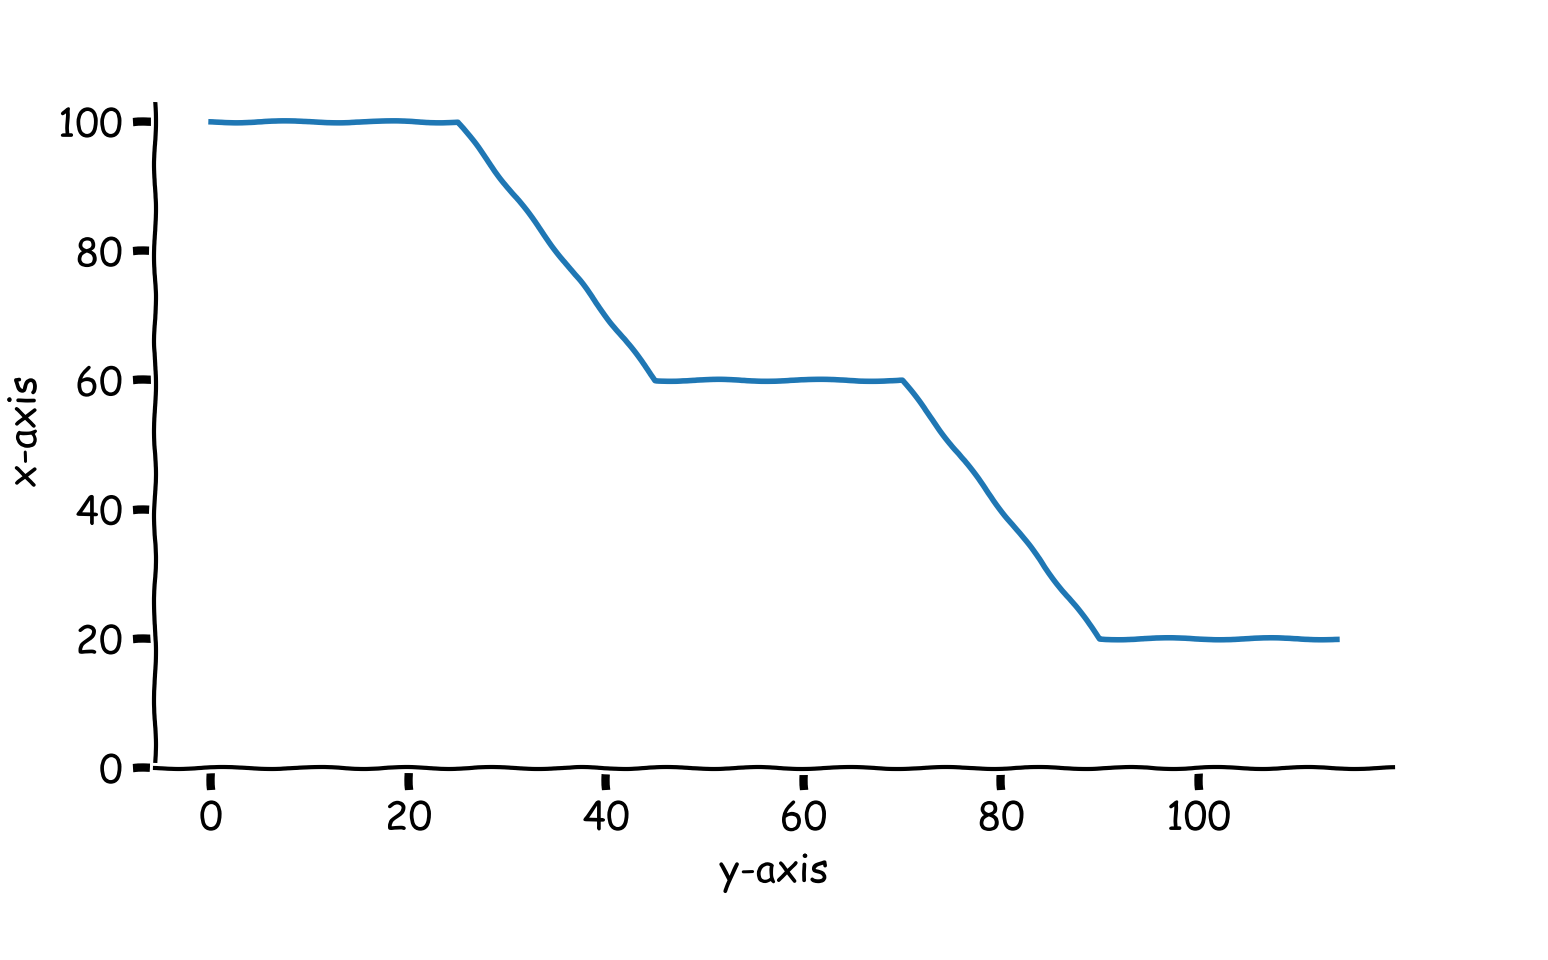
\includegraphics[width=\textwidth]{plateu.png}
    \caption{}
    \label{fig:plateu}
	\end{subfigure}
	%
	\begin{subfigure}[b]{0.3\textwidth}
    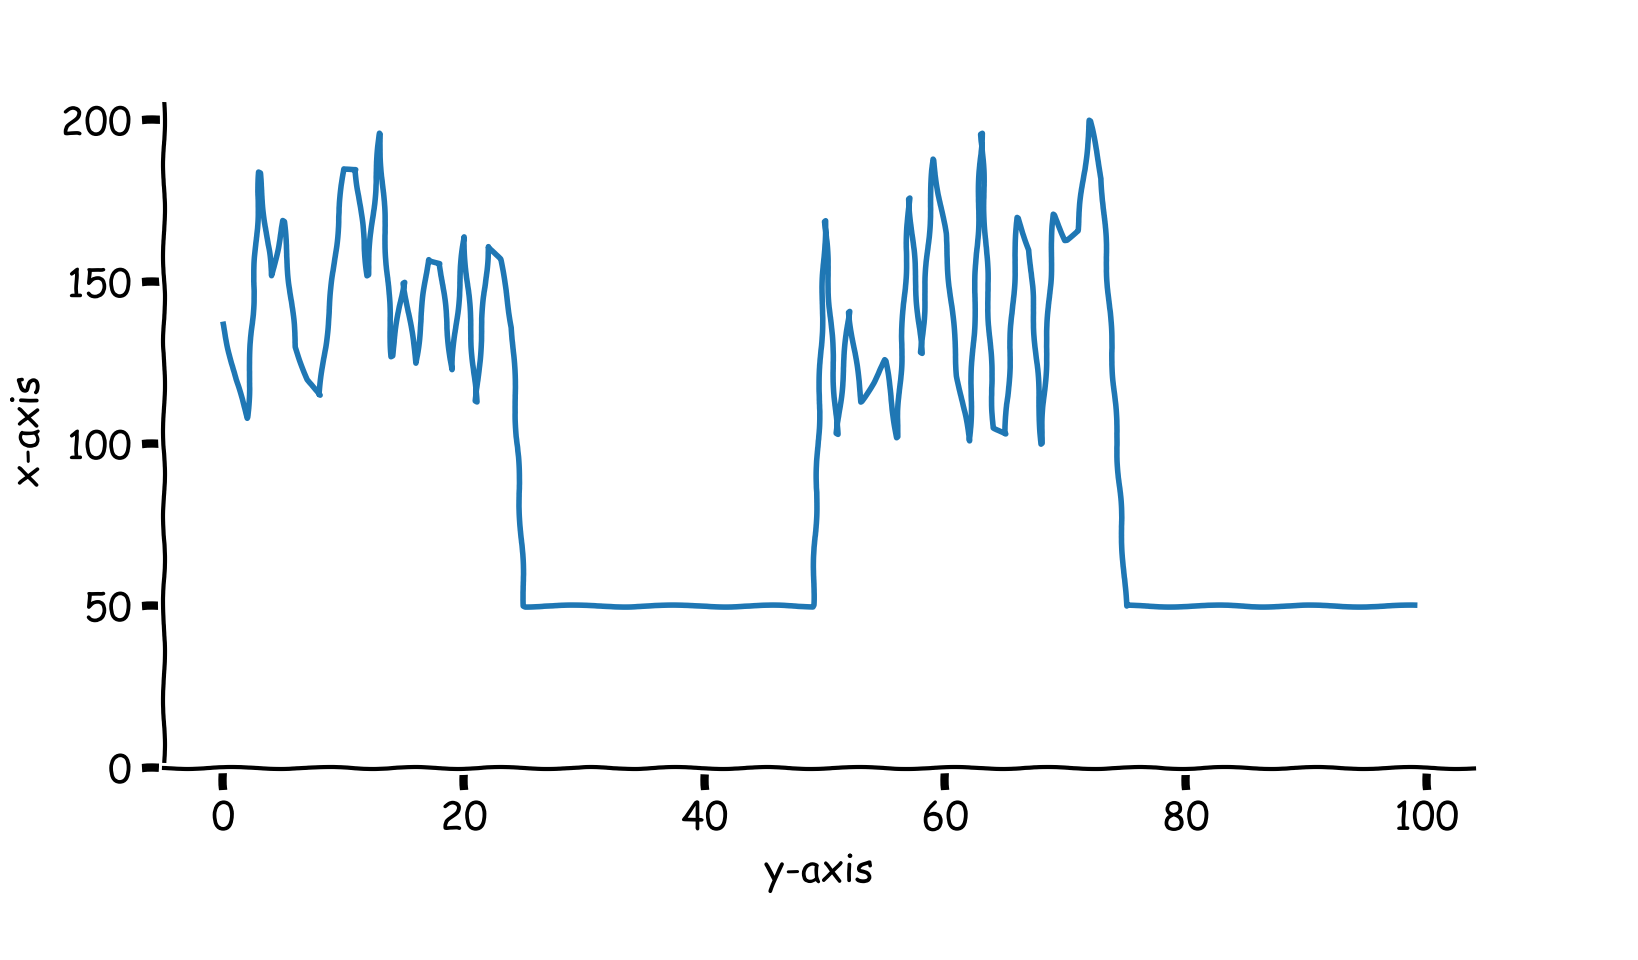
\includegraphics[width=\textwidth]{some_spikes.png}
    \caption{}
    \label{fig:spikes}
	\end{subfigure}
\caption{Graph a) shows plateauing development of values, while graph b) displays spikes in the readings}
\end{figure}

In figure \ref{sub@fig:plateu} we see the sensor outputting stable data around a fixed value, to then experiencing a decrease two times. We want the readings to increase during the data changes, and decrease during the stable plateaus.

In figure \ref{sub@fig:spikes} we see the sensor outputting some data values with sudden spikes in them. For the sake of simplicity, we will assume that our scale has the maximum capacity of 100 kg, and thus can easily discern that any value above this is a false reading. In other contexts, false readings might be harder to detect and handle.

\section{Sensor Failure}
In this paper, we define sensor failure as a sensor giving too many unreliable or false data values to be considered functional. The goal of identifying such a state in an IoT device is to prevent unstable data from being interpreted as valid, which in turn can save the end user from unwanted consequences. Depending on the longevity and purpose of the device, the threshold of when to declare a sensor as failing may differ, especially as this state can be quite fluid. A functional sensor means different things for different devices and applications. A simple way might be to conclude that if x\% of data is considered invalid during the last 24hrs, an alarm should be raised to the device administrator. Complications arise when failures need to be reported quickly, or estimated more thoroughly. It is also possible that the sensor can be temporarily unreliable due to external circumstances, and given enough time, these circumstances might pass. On one extreme you can have a device that reports failures too frequently and bogs down whatever dashboard is handling its status report. On the other, you can have a device taking too long to determine a sensor failure so that false data is believed to be valid in the meantime.

The requirements set on our device state that it has to have some form of self-regulation of when to send these error signals, allowing the sensor some time to recover. If the sensor does not recover within a given timeframe, or outputs too much erroneous data, it will raise an error. The reason for still raising an error even though the device recovered is that the sensor might be in need of maintenance if the \% of invalid data is too high. This all depends on the filtering of invalid data, as well as at what data threshold the device loses effectivity.

\begin{figure}[H]
\centering
	\begin{subfigure}[b]{0.3\textwidth}
    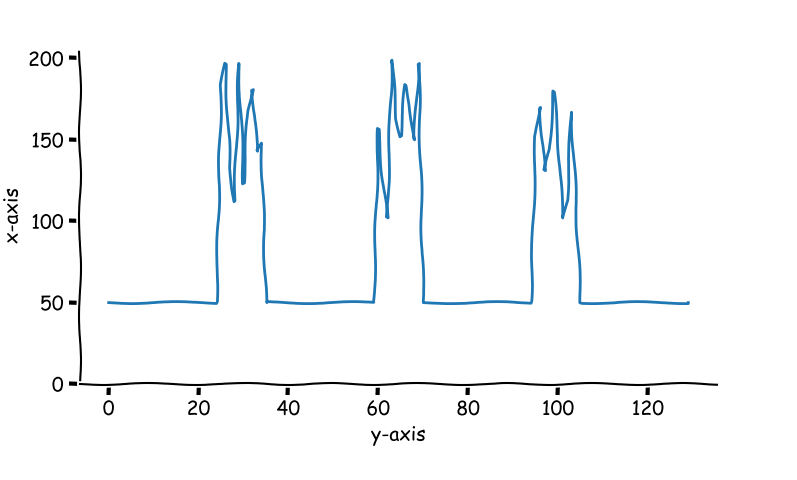
\includegraphics[width=\textwidth]{recover.png}
    \caption{Sensor recovers after some invalid reads}
    \label{fig:recover}
	\end{subfigure}
	%
	\begin{subfigure}[b]{0.3\textwidth}
    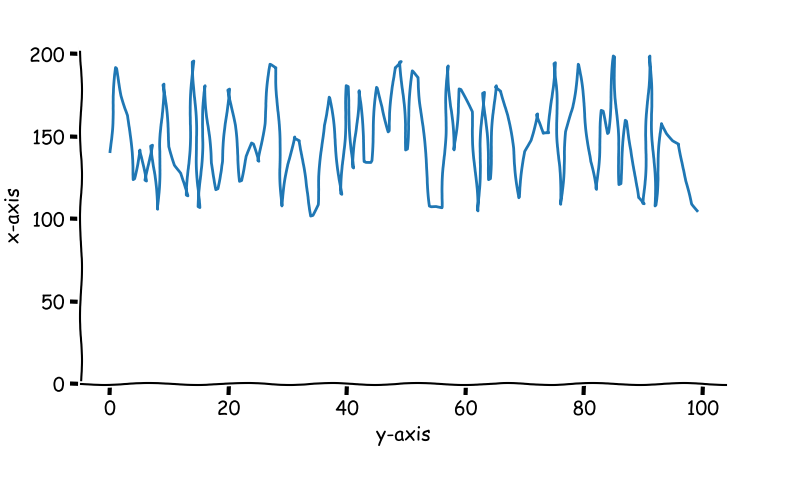
\includegraphics[width=\textwidth]{faulty_data.png}
    \caption{Sensor does not recover after invalid reads}
    \label{fig:no_recover}
	\end{subfigure}
    %
	\begin{subfigure}[b]{0.3\textwidth}
    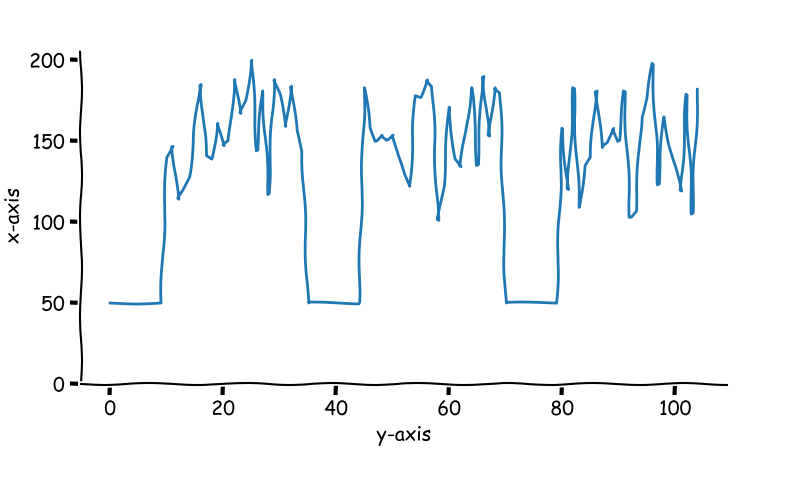
\includegraphics[width=\textwidth]{too_much_invalid.png}
    \caption{Sensor produces too much invalid data}
    \label{fig:too_much_invalid}
	\end{subfigure}
\caption{}
\end{figure}
In figure \ref{sub@fig:recover} the sensor outputs some invalid data, yet it recovers. No errors should be raised.

In figure \ref{sub@fig:no_recover} the sensor does not recover from reading invalid data, and an error should be raised.

In figure \ref{sub@fig:too_much_invalid} the sensor does recover, but still outputs enough invalid data that an error should be raised. 


\section{Sensor Disconnect}
We define a sensor disconnect as when no credible data is being produced at all. If the sensor does not recover, immediate maintenance is needed for any continued functionality. In this device we know that a sensor disconnect results in the value 0.0 being returned at every poll by the microcontroller to the sensor. While this might be a valid read in some scenarios, in a real world application we would probably never get such a stable value at exactly 0.0. Rather, it would fuzz around at maybe between 1.5 and 0.0 (for example). Disregarding this, we can also know that sensor has disconnect if the data values drop to 0.0 at a too quick pace to be a real-world measurement. 

The requirements on this device states that it should raise a disconnect error if the sensor does not recover within a given timeframe.

\begin{figure}[H]
\centering
    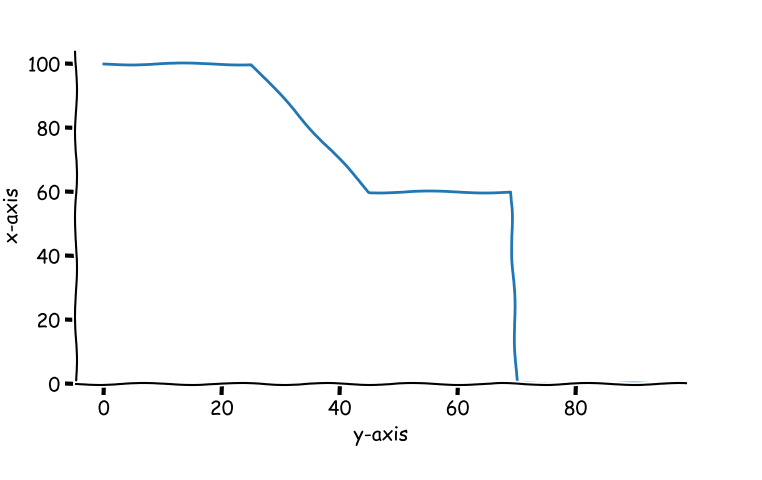
\includegraphics[width=0.3\textwidth]{disconnect.png}
    \caption{The sensor disconnects}
    \label{fig:disconnect}
\end{figure}

In figure \ref{fig:disconnect} the data values drop from 60 to 0 in the span of one data point, which would indicate a sensor disconnect.
